\documentclass[../Thesis_AHoecherl.tex]{subfiles}

\begin{document}

    In this chapter the results produced for the thesis are presented. We will first show with small sample portfolio that numerical Euler allocation of SA-CCR is possible in section \ref{sec:General approach to numerical Euler allocation of SA-CCR}. On these exemplary portfolios we will also point out a couple of observations highlighting how an Euler allocation can offer great insight due to its risk sensitive nature.

    Afterwards, section \ref{sec:Consideration of edge cases} lists scenarios, under which Euler allocation prerequisites are violated and suggests approaches on how to mitigate these issues or proposes a workaround.

    \section{General approach to numerical Euler allocation of SA-CCR\label{sec:General approach to numerical Euler allocation of SA-CCR}}

    In this section we assume, that the minimum transfer amount, variation margin threshold and initial margin threshold as defined in \todo{Enter reference} are all 0. This means, that the margin calculated by the used variation margin and initial margin model is entirely incorporated in the SA-CCR model for EAD calculation.

    The reason for this is, that assumptions other than 0 for the thresholds and MTA generally violate the homogeneity prerequisite for Euler allocation. In practice, this is a strong and somewhat unrealistic assumption as for example an initial margin threshold of 50Mn is usual for bilateral portfolios as it is the highest amount allowed by the regulator \todo{Reference to where this is stated}. Due to the high practical relevance the impact of thresholds and MTA on Euler allocation is analyzed in detail in section \ref{sec:Consideration of edge cases}.   

    \subsection{Exemplary allocation of SA-CCR for a small portfolio of equity options}

    In this section we analyze an Euler allocation of a small portfolio of equity options. The detailed computation steps are demonstrated in appendix \ref{sa-ccr-euler-allocation-of-exemplary-equity-portfolio}. 
    First, we consider a portfolio consisting of two million call options and three million put option on Adidas. All options are struck at the current stock price and long. Obviously, the two positions are in a hedge relation and being at the money long options both positions do have a significant, positive present value.
    
    With ISDA-SIMM and SA-CCR portfolio risk measures introduced in \todo{add reference} and considering different margining approaches we can calculate portfolio risk measure values displayed the portfolio risk measure column of table \ref{tab:2TradeEquityResults}.
    % Table generated by Excel2LaTeX from sheet 'Sheet1'
    \begin{table}[htbp]
        \centering
        \begin{tabular}{l||r|r|r}
                & 2Mn ADS Call & 3Mn ADS Put & Portfolio Risk Measure\\
                \toprule
        SIMM  & -33.75\% & 133.75\% & 14,231,564 USD \\
        No margin & 99.21\% & 0.79\% & 37,643,536 USD \\
        VM only & 232.47\% & -132.47\% & 3,519,458 USD \\
        VM+IM & 622.10\% & -522.10\% & 345,874 USD \\
        \end{tabular}%
        \caption{}
        \label{tab:2TradeEquityResults}%
    \end{table}%
    It can be seen that incorporation of the variation margin significantly drops the portfolio EAD. The reason for this is that the RC in formula \todo{ref needed} drops from 


    Figure \ref{fig:C for ITM IRS} also showcases the trivial result that the Variation Margin is a homogeneous function - the value of the trade scales linearly with the notional.
    
    Critically, this result can also be transferred to any SA-CCR allocation approach that would treat C as an externally given constant value as locally, treating C as a constant value is the same as consideration of a \gls{MTA}. 
    In both cases the slope of C is zero.  

    \section{Consideration of edge cases\label{sec:Consideration of edge cases}}

    While numerical Euler allocation of SA-CCR and ISDA SIMM is generally possible as shown in section \ref{sec:General approach to numerical Euler allocation of SA-CCR} a couple of cases can be identified, in which Euler allocation fails since its prerequisites of homogeneity and differentiability are violated.
    Both, ISDA SIMM and SA-CCR are complex, convoluted formulas, make it different to make general observations on differentiability and homogeneity.
    In fact, we will see that depending on the portfolio and parametrization of the collateral agreement, both ISDA SIMM and SA-CCR are not homogeneous risk measures, and that they are both occasionally not partially differentiable w.r.t. position size.

    In this section, all identified cases under which prerequisites for Euler allocation are violated are presented and for some a workaround is presented to allow nevertheless for risk sensitive and naturally additive allocation.

    \subsection{Allocation when an ISDA-SIMM liquidity threshold is exceeded\label{sec:Allocation when an ISDA-SIMM liquidity threshold is exceeded}}
    
    As pointed out in section \ref{sec:Euler allocation} a risk measure needs to exhibit positive homogeneity of degree 1 to be able to perform an Euler allocation.
    This precondition is violated if a liquidity threshold of the ISDA SIMM model is exceeded.

    We can show this by exploring whether ISDA SIMM does exhibit positive homogeneity for a minimal example.

    For this we set up an USD Libor IRS with ten years time to maturity and a notional of 200 billion USD. This is our initial portfolio $\mathbf{u}$. ISDA SIMM would fulfill the required positive homogeneity condition if $a \rho(\mathbf{u}) = \rho(a \mathbf{u}$ for $a>0$. In figure \ref{fig:homogeneity of ISDA SIMM} $\rho(a\mathbf{u})$ is plotted for $0<a\leq 2$ in blue. 
    \begin{figure}
        \centering
        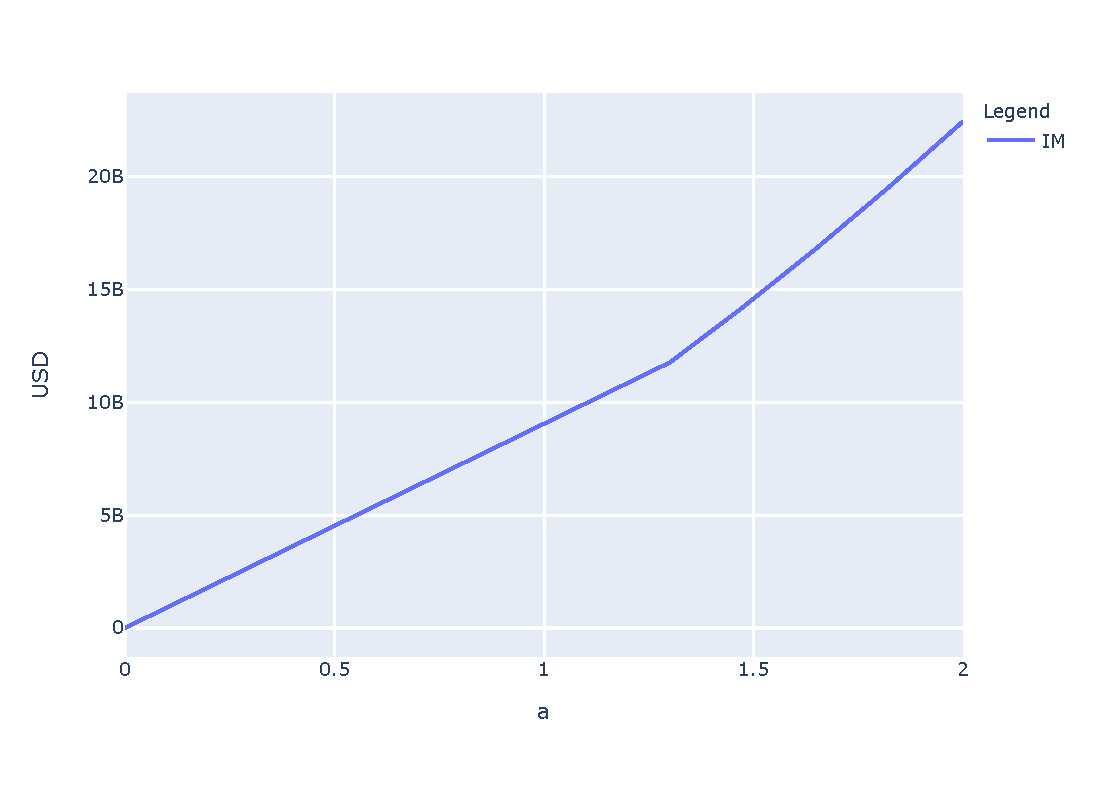
\includegraphics{Graphics/ISDA_SIMM_homogenity.pdf}
        \caption{}
        \label{fig:homogeneity of ISDA SIMM}
    \end{figure}
    The function exhibits homogeneity for $0<a<1.4$ \todo{find the exact point where homogeneity breaks} but not for higher $a$. 
    The reason for this is, that at this point the concentration risk charge of ISDA SIMM does kick in.
    The concentration risk for interest rate risks for our minimal example is defined as \cite[Article 7.b]{SIMM}
    \begin{align*}
        CR = \max\left(1,\left(\frac{\lvert\sum{s}\rvert}{T}\right)^{1/2}\right)
    \end{align*}
    with $s$ being the sensitivities against USD interest rate risk and T being 230Mn USD as specified in \cite[Article 74]{SIMM}. Due to subsequent variance-covariance aggregation the concentration risk impacts the calculated IM as
    \begin{align*}
        IM_{\text{with conc. risk}} = CR^2 \cdot IM_{\text{without conc. risk}}
    \end{align*}
    This causes the change in slope and implied loss of homogeneity visible in figure \ref{fig:homogeneity of ISDA SIMM}. If the portfolio would consist of a more diverse set of risk factors than the minimal example displayed in figure \ref{fig:homogeneity of ISDA SIMM} the associated concentration risk would kick in at different levels of $a$.
    The slope of the function would increase with each additional concentration risk not being floored at one any more. 
    
    It is important to note that as soon as the sensitivity against a single risk factor in the portfolio is above the concentration threshold the ISDA SIMM risk measure does not exhibit homogeneity anymore.

    Even a trivial example with just one trade is sufficient to show that Euler allocation does not work in the inhomogeneous part of the ISDA SIMM equation.
    For this, we compare two sample portfolios one consisting of one USD IRS with 200 bn notional and one consisting of one USD IRS with 400 bn notional.
    Critically, the second portfolio is penalized by the model since its USD IRS risk is too large. We calculate the Euler calculation with a forward finite difference approach as displayed in equation \ref{eq:forward difference}.

    Assuming that we calculate the finite difference with an $\epsilon = 0.0001$ this means that we calculate the ISDA SIMM of an IRS with 200Bn notional ($SIMM_{200Bn}$) and the ISDA SIMM of an equivalent IRS with 200.02 Bn notional ($SIMM_{200.02Bn}$) and this yields an Euler allocation to this trade as
    \begin{align*}
        \frac{SIMM_{200.02Bn} - SIMM_{200Bn}}{0.0001} = 9.04Bn
    \end{align*}
    We can see in figure \ref{fig:homogeneity of ISDA SIMM} that this value is both, the slope and the IM value at $a = 1$. The portfolios IM was correctly fully allocated to the single trade of which it consists. 
    
    However, performing the same calculation for an equivalent IRS with 400Bn notional yields
    \begin{align*}
        \frac{SIMM_{400.04Bn} - SIMM_{400Bn}}{0.0001} = 33.67Bn
    \end{align*}
    again, we can refer to figure \ref{fig:homogeneity of ISDA SIMM} to check if this is a reasonable allocation result. As $a=1$ represents the IM charge for investing 200Bn of notional in the IRS, $a=2$ represents an investment of 400Bn notional. The associated IM is just 22.44Bn - allocating 33.67Bn of the risk measure to the only trade in the portfolio is therefore clearly wrong. The Euler allocation of 33.67Bn can also be read off figure \ref{fig:homogeneity of ISDA SIMM} - it is the slope at $a=2$ times two.

    Euler allocation of SA-CCR also does not work if the calculated C does not exhibit homogeneity, i.e. if a concentration risk threshold of the ISDA-SIMM model is exceeded. Again using the 400Bn IRS from \ref{Allocation of initial margin} we calculate an EAD\textsubscript{400Bn IRS} of 843.5Mn but, despite not applying an MTA, Euler allocation yields a vastly different amount of $ \frac{\text{EAD\textsubscript{200.02Bn IRS}}-\text{EAD\textsubscript{200Bn IRS}}}{0.0001} = 201.0Mn $. If for a given portfolio C does not exhibit homogeneity, neither does SA-CCR and therefore Euler allocation of SA-CCR is not possible for such portfolios. \todo{Paragraph needs to be tidied up as it has been relocated}

    As can already seen by the notional of the exemplary trade, the liquidity thresholds imposed by ISDA-SIMM are relatively high and will not be exceeded by the majority of bilateral portfolios.

    \todo{Insert explanation that this can't really be fixed.}

    \subsection{Incorporation of a minimum transfer amount and threshold}

    To allocate \gls{SA-CCR} under consideration of margining, the available collateral $C$ is of special interest. As pointed out in table \ref{tab:Margin in SA-CCR} depending on the margining approach, C can be calculated as $C = \text{VM}$ or $C = \text{VM} + \text{IM}_{\text{received}}$.

    The actually exchanged collateral, however has to be calculated under consideration of the threshold and minimum transfer amount as displayed in equation \ref{eq:C} \todo{Fix reference}. With this consideration of threshold and minimum transfer amount $C$ is not a homogeneous function. 

    \begin{figure}
        \centering
        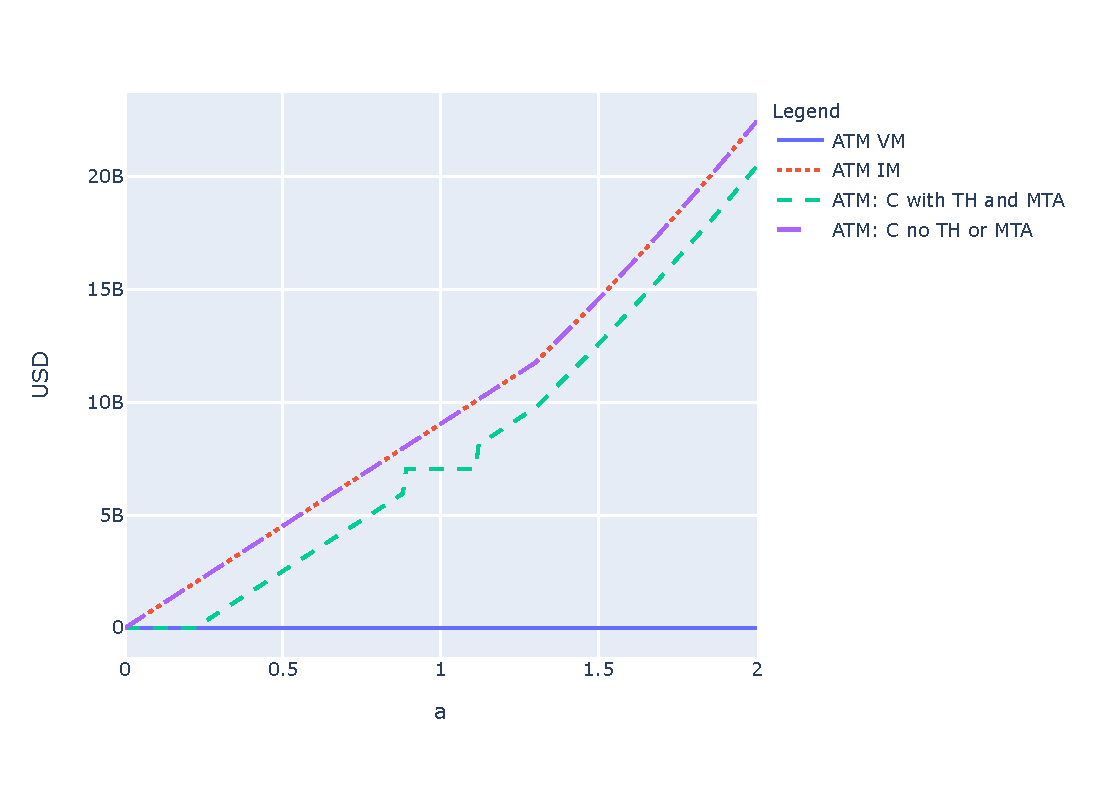
\includegraphics{Graphics/C_and_its_components_for_ATM_IRS.pdf}
        \caption{VM, IM, C and C under consideration of TH and MTA for a portfolio consisting of a single at the money interest rate swap. Values are calculated based on different notionals invested in the IRS with $a=1$ referring to a notional of 200Bn USD. More details on creation can be found in Appendix \ref{homogeneity-of-c-for-a-single-trade-portfolio}.}
        \label{fig:C for ATM IRS}
    \end{figure}

    \begin{figure}
        \centering
        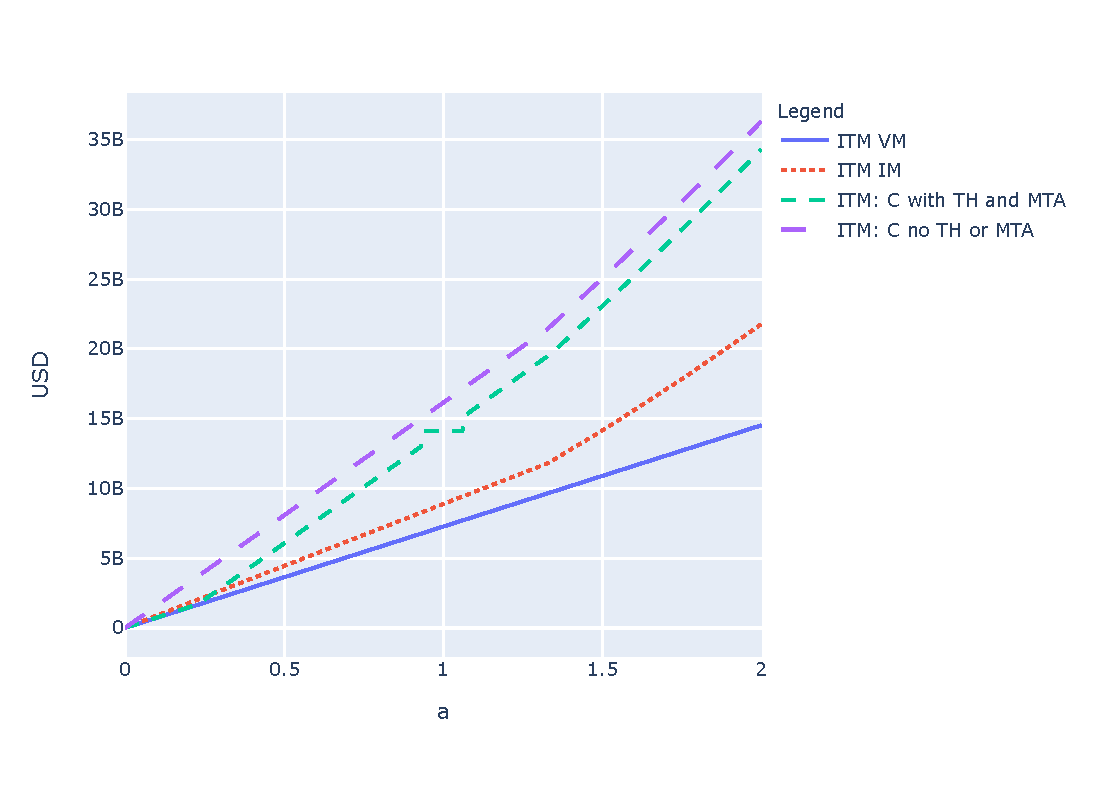
\includegraphics{Graphics/C_and_its_components_for_ITM_IRS.pdf}
        \caption{Same as figure \ref{fig:C for ATM IRS} but for an in the money trade with an payer interest rate at 2\% which is below par.}
        \label{fig:C for ITM IRS}
    \end{figure}

    This can exemplary seen in figures \ref{fig:C for ATM IRS} and \ref{fig:C for ITM IRS}. These figures display $C$ for an at the money 10Y USD interest swap and the same swap with a lower fixed rate making it an in the money swap. Again, a very high notional of 200 Bn is chosen to showcase the concentration risk charge of ISDA SIMM and the threshold and minimum transfer amount have also been chosen to be very high at 2Bn and 1Bn USD.

    \subsubsection{Incorporation of a minimum transfer amount}

    \todo{This paragraph probably needs to be removed} To be able to calculate an Euler allocation of SA-CCR one has to calculate C for use in \ref{eq:multiplier} without recognition of the minimum transfer amount as the $C_{calc}$ as defined in equation \ref{eq:C_calc}.
    \begin{align}
        \label{eq:C_calc}
        C_{calc} &= VM + IM_{rec}
    \end{align}
    
    If only a MTA but no threshold is in place, no further adjustment is necessary.
    This can exemplary been seen in the next example.
    Again, similar to the exemplary calculation in section \ref{sec:Allocation when an ISDA-SIMM liquidity threshold is exceeded} it can be shown with a trivial example, that Euler allocation of SA-CCR is not possible under recognition of a \gls{MTA}. 
    For this we consider the same 200Bn \gls{IRS} as in section \ref{sec:Allocation when an ISDA-SIMM liquidity threshold is exceeded}. We assume that the currently posted margin is 9.04Bn which is the calculated ISDA-SIMM margin. 
    Setting $C$ at 9.04Bn in \ref{eq:multiplier} and then calculating the SA-CCR EAD for this single IRS \todo{as specified in ...} yields an regulatory EAD of 582.8Mn USD. Any natively additive allocation should allocate this full amount to the IRS.
    The \gls{VM} is zero as the IRS is struck at par.
    \begin{table}[htbp]
        \label{tab:Allocate SA-CCR with MTA calculation}
        \centering
            \begin{tabular}{c|c|c}
                & $\text{SA-CCR}_{\text{MTA}}$ & $\text{SA-CCR}_{\text{No \gls{MTA}}}$ \\
                \toprule
                Initial C & 9038.2Mn & 9038.2Mn \\
                \midrule
                EAD\textsubscript{200Bn IRS} & 582.8Mn & 582.8Mn \\
                \midrule
                C\textsubscript{200Bn IRS} & 9038.2Mn & 9038.2Mn \\
                \midrule
                C\textsubscript{200.02Bn IRS} & 9038.2Mn & 9039.1Mn \\
                \midrule
                EAD\textsubscript{200.02Bn IRS} & 583.0Mn & 582.9Mn \\
                \midrule
                $\frac{\text{EAD\textsubscript{200.02Bn IRS}}-\text{EAD\textsubscript{200Bn IRS}}}{0.0001}$ & 1425.3Mn & 582.8Mn  \\
            \end{tabular}%
        \caption{Numerical Euler allocation of SA-CCR with and without consideration of a minimum transfer amount for an example of a portfolio with a single 200Bn notional IRS. Euler allocation is only successful if the \gls{MTA} is not considered for the recalculation of the received margin C. A threshold of 0 is assumed.}
    \end{table}
    In table \ref{tab:Allocate SA-CCR with MTA calculation} we assume that the initially received collateral is the currently calculated collateral. 
    When calculating the Euler allocation with a forward difference in line with \ref{eq:forward difference} the received collateral when rising the notional to 200.02Bn increases when no MTA is assumed while it remains unchanged with consideration of an MTA. 
    Ultimately, this difference leads to a correct allocation of the entire EAD to the single IRS with the \emph{No MTA} approach while the \emph{MTA} approach obviously yields a wrong result by allocating 244\% of the portfolios EAD to its only trade.

    \subsubsection{Incorporation of a VM threshold\label{sec:Incorporation of a VM threshold}}

    \subsubsection{Incorporation of an IM threshold\label{sec:Incorporation of an IM threshold}}

    Consideration of the threshold is challenging. When calculating $C$ with a threshold, $C$ does not exhibit homogeneity and an allocation will fail. On the other hand, when calculating $C$ without threshold the considered margin is to high and the sum of allocated EAD will be too low.
    One solution to this is to first allocate the SA-CCR assuming the threshold is 0 and then scaling up the allocation by $EAD_{TH = 0} \ EAD$ where $EAD_{TH = 0}$ is the calculated SA-CCR EAD assuming a zero threshold and $EAD$ is the actual SA-CCR EAD.


    \subsection{Allocation of hedged portfolios}

    As pointed out in \ref{Allocation of Risk Measures} Euler allocation is a risk sensitive allocation and as such does generally attribute negative contributions to trades that are decreasing the risk of the portfolio. If we consider a portfolio of a 200Mn payer IRS, an equivalent 100Mn receiver IRS and 1Mn long stock call options we yield the result depicted in \ref{tab:hedge trade sample results} when calculating the Euler allocation numerically with a forward difference.
    \begin{table}[htbp]
        \label{tab:hedge trade sample results}
        \centering
            \begin{tabular}{c|c|c}
                & SA-CCR & ISDA SIMM \\
                \toprule
                IRS\textsubscript{100Mn Rec} & -246k & -4.52Mn \\
                \midrule
                IRS\textsubscript{200Mn Pay} & 493k & 9.04Mn \\
                \midrule
                Equity Option & 1.30Mn & 6.95Mn \\
                \bottomrule
                Sum of allocations & 1.54Mn & 11.47Mn \\
                \midrule
                Portfolio risk measure & 1.54Mn & 11.47Mn \\
            \end{tabular}%
        \caption{}
    \end{table}
    The 100Mn receiver IRS partially hedges the risk induced by the 200Mn payer IRS. 
    Both, the ISDA SIMM and the SA-CCR model do not recognize any hedge effects across asset classes and therefore the risk associated with the equity option is completely independent from the two IRS trades. 
    Appropriately, a negative IM and EAD is allocated to the smaller IRS trade and the allocation exhibits native additivity as the sum of the allocation of the three trades coincides with the risk measures of the portfolio.
    
    However, an allocation 

    \begin{table}[htbp]
        \label{tab:EAD perfect hedge}
        \centering
            \begin{tabular}{c|c|c|c}
                & Forward & Central & Backward \\
                \toprule
                IRS\textsubscript{200Mn Rec} & 188k & 0k & -188k \\
                \midrule
                IRS\textsubscript{200Mn Pay} & 188k & 0k & -188k\\
                \midrule
                Equity Option & 1.32Mn & 1.32Mn & 1.32Mn\\
                \bottomrule
                Sum of allocations & 1.69Mn & 1.32Mn & 944k \\
                \midrule
                Portfolio risk measure & \multicolumn{3}{c}{1.32Mn} \\
            \end{tabular}%
        \caption{}
    \end{table}

    \begin{table}[htbp]
        \label{tab:IM perfect hedge}
        \centering
            \begin{tabular}{c|c|c|c}
                & Forward & Central & Backward \\
                \toprule
                IRS\textsubscript{200Mn Rec} & 4.52Mn & 0.00Mn & -4.52Mn \\
                \midrule
                IRS\textsubscript{200Mn Pay} & 4.52Mn & 0.00Mn & -4.52Mn \\
                \midrule
                Equity Option & 6.95Mn & 6.95Mn & 6.95Mn \\
                \bottomrule
                Sum of allocations & 15.99Mn & 6.95Mn & -2.09Mn \\
                \midrule
                Portfolio risk measure & \multicolumn{3}{c}{6.95Mn}  \\
            \end{tabular}%
        \caption{}
    \end{table}

\end{document}